\documentclass[10pt,x11names,table]{beamer}

\usetheme[progressbar=frametitle]{metropolis}
\usepackage{appendixnumberbeamer}
\usepackage{xcolor}

\usepackage{polyglossia}
\setmainlanguage{spanish}

\usepackage{listings}

\usepackage{booktabs}
\usepackage[scale=2]{ccicons}

\usepackage{pgfplots}
\usepgfplotslibrary{dateplot}

%ANIMACIONES
\usepackage{animate}
\usepackage{graphicx}
\usepackage[caption=false]{subfig}

\usepackage{xspace}

\newcommand*{\eg}{e.g.\@\xspace}
\newcommand*{\ie}{i.e.\@\xspace}

\let\oldquote\quote
\let\endoldquote\endquote
\renewenvironment{quote}[2][]
  {\if\relax\detokenize{#1}\relax
     \def\quoteauthor{#2}%
   \else
     \def\quoteauthor{#2~---~#1}%
   \fi
   \oldquote}
  {\par\nobreak\smallskip\hfill(\quoteauthor)%
   \endoldquote\addvspace{\bigskipamount}}
   
\usepackage{wrapfig}

\usepackage{subfig}
\usepackage{hyperref}
\usepackage{multicol}

\setbeamertemplate{bibliography item}[text]

\usepackage[font=small,skip=0pt, labelformat=empty]{caption}

\usepackage{dirtytalk}
\usepackage[acronym]{glossaries}
\makeglossaries

\newacronym{ae}{AE}{Autoencoder}
\newacronym{ai}{AI}{Artificial Intelligence}
\newacronym{brief}{BRIEF}{Binary Robust Independent Elementary Features}
\newacronym{cnn}{CNN}{Convolutional Neural Network}
\newacronym{diffit}{DiffiT}{Diffusion Vision Transformer}
\newacronym{dl}{DL}{Deep Learning}
\newacronym{fast}{FAST}{Features from Accelerated Segment Test}
\newacronym{gan}{GAN}{Generative Adversarial Network}
\newacronym{gpu}{GPU}{Graphics Processing Unit}
\newacronym{ilsvrc}{ILSVRC}{ImageNet Large Scale Visual Recognition Challenge}
\newacronym{nlp}{NLP}{Natural Language Processing}
\newacronym{nn}{NN}{Neural Network}
\newacronym{ocr}{OCR}{Optical Character Recognition}
\newacronym{sift}{SIFT}{Scale-Invariant Feature Transform}
\newacronym{slam}{SLAM}{Simultaneous Localization and Mapping}
\newacronym{surf}{SURF}{Speeded-Up Robust Features}
\newacronym{vae}{VAE}{Variational Autoencoder}
\newacronym{vgg}{VGG}{Visual Geometry Group}
\newacronym{vit}{ViT}{Vision Transformer}
\newacronym{yolo}{YOLO}{You Only Look Once}
\subtitle{Métodos Generativos, curso 2024-2025}

\date{\today}
\author{Guillermo Iglesias, guillermo.iglesias@upm.es \newline
Jorge Dueñas Lerín, jorge.duenas.lerin@upm.es  \newline
Félix Fuentes Hurtado, felix.fuentes@upm.es}

\institute{Escuela Técnica Superior de Ingeniería de Sistemas Informáticos | UPM \newline
\hbox{} \newline \ccbysa \hspace{0.1pt} \ccNonCommercial}

%%%%%%%%%%%%%%%%%%%%%%%%%%%%%%%%%%%%%       
\title{Repaso de redes neuronales artificiales}

\begin{document}
\maketitle

\section{Repaso de conceptos básicos de redes neuronales}

\begin{frame}{Redes neuronales: concepto general}
Una \alert{red neuronal} es un sistema matemático capaz de aprender ha realizar predicciones a partir de unos datos de entrada, fue propuesta por McCulloch y Pitts en 1943\cite{mcculloch1943logical}, se basaba en \alert{imitar} el comportamiento de una neurona biológica.

\begin{itemize}
    \item Toma ciertos \alert{estímulos} de entrada, los procesa y genera una nueva salida.
    \item En el caso biológico los estímulos provienen de \alert{impulsos nerviosos}, mientras que en el caso de las neuronas artificiales esto es replicado a través de cálculos matemáticos.
\end{itemize}

\begin{figure}
    \centering
    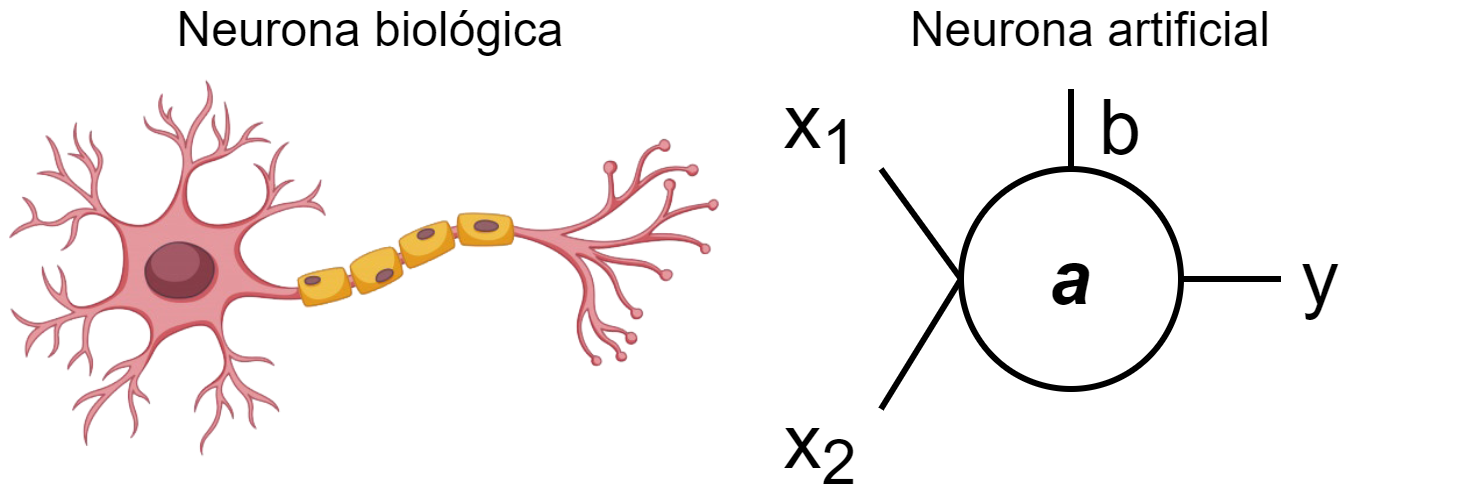
\includegraphics[width=0.7\textwidth]{figures/Tema 3/Neurona_Biologica_Artificial.png}
\end{figure}    
\end{frame}

\begin{frame}{Redes neuronales: concepto general}
Una \alert{neurona artificial} realiza cálculos matemáticos para transformar ciertos valores numéricos.
Para dicha labor, existen diversos \alert{elementos} dentro de una neurona artificial:
\begin{columns}[c]
\centering
\begin{column}{0.7\textwidth}
    \begin{itemize}
    \item \alert{Entradas} ($ x_{i} $): Introducen valores numéricos en la neurona
    \item \alert{Salida} ($ y $): Suministra la salida de la neurona
    \item \alert{Pesos} ($ w_{i} $): Son parámetros capaces de cambiar, realizan el aprendizaje de la neurona
    \item \alert{Bias} ($ b $): Realiza la misma función que cualquier otro peso, pero el valor de su entrada es \alert{siempre} 1
    \item \alert{Función de activación} ($ a $): Es una función que participa en el cálculo de la salida de la neurona
    \end{itemize}
\end{column}
\begin{column}{0.3\textwidth}
    \centering
    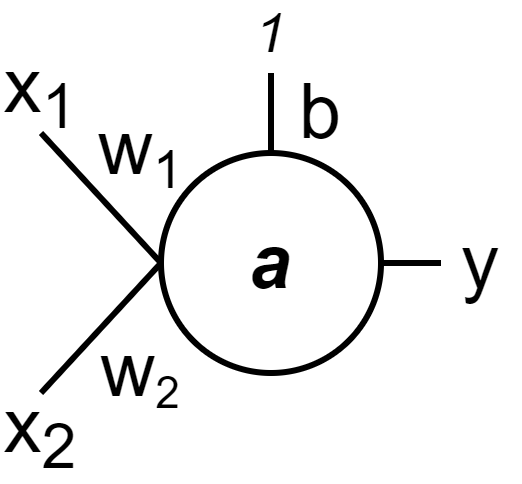
\includegraphics[width=\textwidth]{figures/Tema 3/Neurona_Componentes.png}
\end{column}
\end{columns}
\end{frame}

\begin{frame}{Redes neuronales: bias}
El \alert{bias} (sesgo en Español) permite que la red neuronal pueda ajustar mejor sus predicciones. 
\begin{columns}[c]
\centering
\begin{column}{0.4\textwidth}
    \centering
    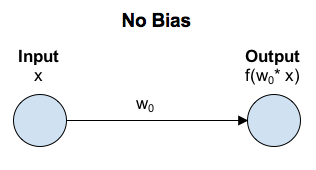
\includegraphics[width=\textwidth]{figures/Introduccion/bias-no.png}
    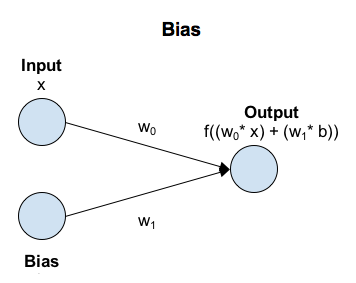
\includegraphics[width=\textwidth]{figures/Introduccion/bias-si.png}
\end{column}
\begin{column}{0.4\textwidth}
    \centering
    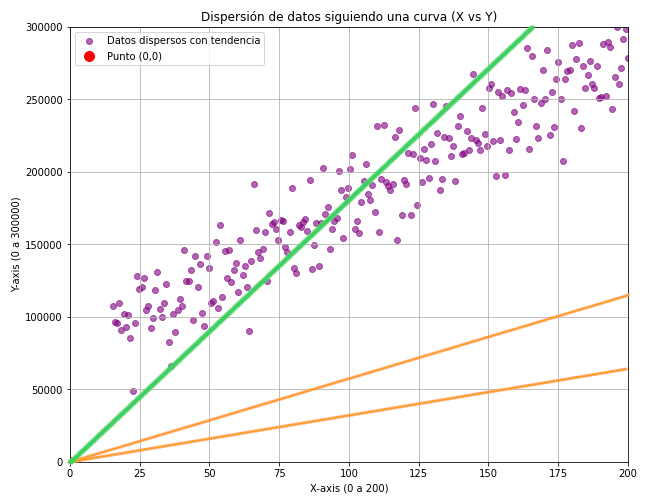
\includegraphics[width=\textwidth]{figures/Introduccion/bias-no-data.png}
    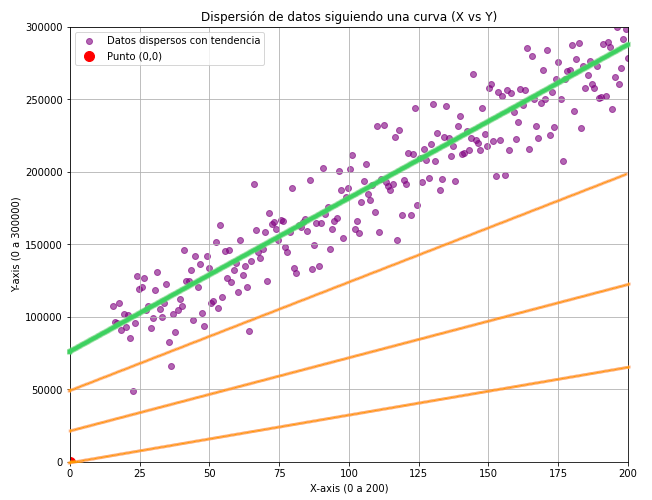
\includegraphics[width=\textwidth]{figures/Introduccion/bias-si-data.png}
\end{column}
\end{columns}

\scriptsize{
Fuente izq: https://www.pico.net/kb/the-role-of-bias-in-neural-networks/
}

\end{frame}

\begin{frame}{Redes neuronales: activación}
Capas de activación. En salida.
\newline

\begin{columns}[c]
\centering
\begin{column}{0.4\textwidth}
    \centering
    \includegraphics[width=\textwidth]{figures/Introduccion/clasificación.png}
    \scriptsize{Fuente Coursera}
    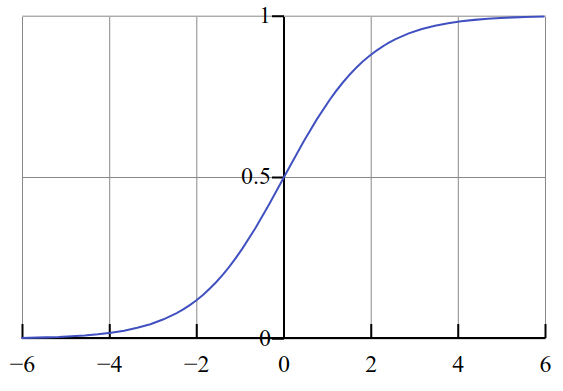
\includegraphics[width=\textwidth]{figures/Introduccion/sigmoid_graph.png}
    \scriptsize{Wikipedia}
\end{column}
\begin{column}{0.4\textwidth}
    \centering

    \textbf{Sigmoid}
    \begin{equation}
     y = \frac{1}{1 + e^{-z}}
    \end{equation}
    
    \vspace{0.5cm}
    
    \textbf{Ejemplo}
    \begin{equation}
     y = \frac{1}{1 + e^{-(3*x-2)}}
    \end{equation}

    \vspace{0.5cm}
    
    \href{https://www.desmos.com/calculator/ctrsgcjd8n}{Calculadora gráfica}
\end{column}
\end{columns}

\end{frame}

\begin{frame}{Redes neuronales: activación}
Capas de activación. No linealidad.

\begin{columns}[c]
\centering
\begin{column}{0.3\textwidth}
    \centering
    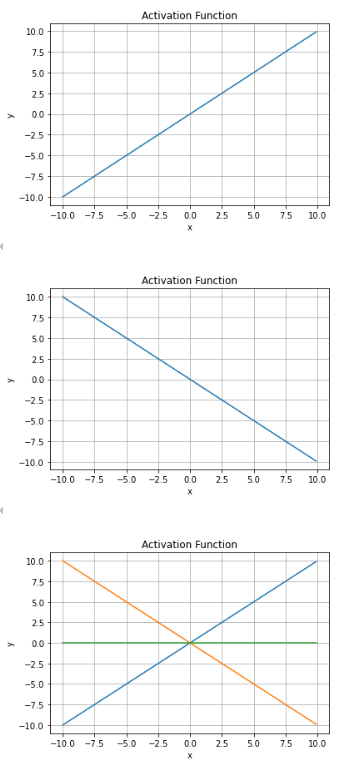
\includegraphics[width=\textwidth]{figures/Introduccion/combilineal.png}
\end{column}
\begin{column}{0.3\textwidth}
    \centering
    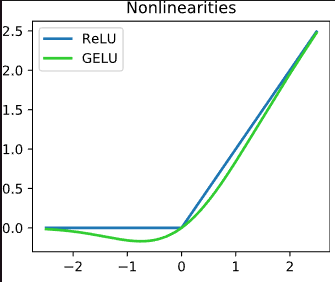
\includegraphics[width=\textwidth]{figures/Introduccion/relu.png}
    \scriptsize{Wikipedia}
\end{column}
\begin{column}{0.3\textwidth}
    \centering
    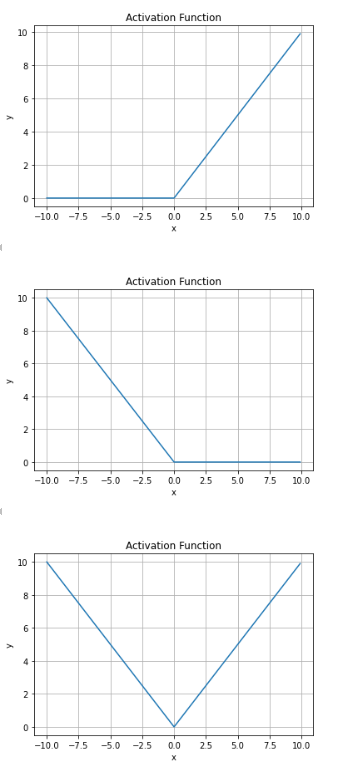
\includegraphics[width=\textwidth]{figures/Introduccion/combinolineal.png}
\end{column}
\end{columns}
\end{frame}


\begin{frame}{Redes neuronales: activación}
Capas de activación. No linealidad. 3D

\begin{columns}[c]
\centering
\begin{column}{0.5\textwidth}
    \centering
    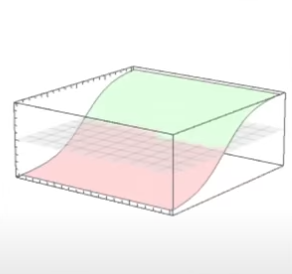
\includegraphics[width=0.8\textwidth]{figures/Introduccion/activacion_3d.png}
\end{column}
\begin{column}{0.5\textwidth}
    \centering
    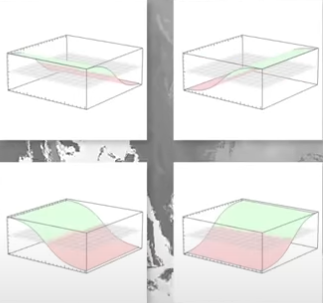
\includegraphics[width=0.8\textwidth]{figures/Introduccion/activacion_3d_varias.png}
\end{column}
\end{columns}

\centering
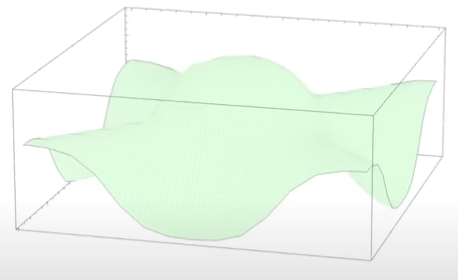
\includegraphics[width=0.4\textwidth]{figures/Introduccion/activacion_3d_combi.png}

\scriptsize{DotCSV}

\end{frame}

\begin{frame}{Redes neuronales: entrenamiento}
El entrenamiento de las redes neuronales se puede dividir en tres fases: 
\begin{columns}[c]
\begin{column}{0.49\textwidth}
\begin{itemize}
    \item \alert{Predicción:} calculamos para las entradas la predicción de valor de salida de la red.
    \item \alert{Calculo de error:} con la predicción y el resultado que queremos obtener calculamos el error obtenido.
    \item \alert{Ajuste de pesos:} con el error se reajustan los parámetros de la red.
\end{itemize} 
\end{column}

\begin{column}{0.49\textwidth}
\begin{figure}
\centering
    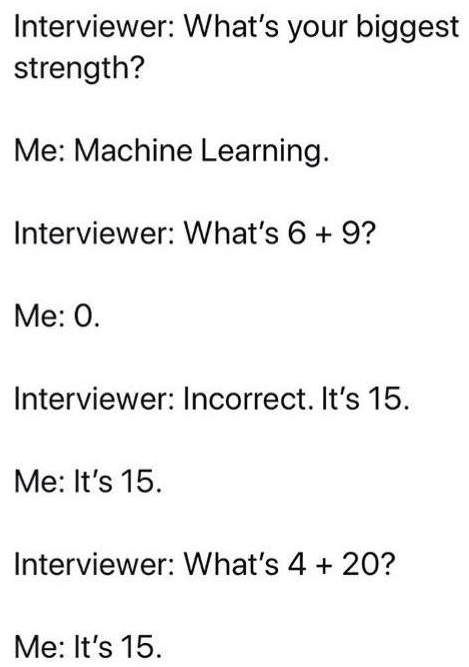
\includegraphics[width=0.9\textwidth]{figures/Tema 3/jokeML.png}
\end{figure}
\end{column}
\end{columns}
\end{frame}

\begin{frame}{Algoritmo de propagación}
La fase de \alert{predicción} de una red neuronal se realiza a través del algoritmo de \alert{propagación}.

Este se encarga de procesar la \alert{entrada} y generar la \alert{salida} correspondiente.

Para ello, la computación de cada \alert{neurona} es la siguiente:
\begin{itemize}
    \item Cada entrada $x_{i}$ es \alert{multiplicada} por el valor de su peso correspondiente $w_{i}$.
    \item La entrada de \textit{bias} \alert{siempre} es \say{1}, y se multiplica por su peso correspondiente (a veces indicado como $w_{0}$).
    \item Todas las \alert{entradas} de la neurona se combinan haciendo una \alert{suma} de todas ellas, de tal manera que se realiza una \alert{combinación lineal}.
    \item El resultado de la combinación lineal se pasa por una \alert{función no lineal} para generar la \alert{salida} de la neurona.
\end{itemize}
\end{frame}

\begin{frame}{Algoritmo de propagación}
La ecuación que define este \alert{proceso} es la siguiente:
\setcounter{equation}{0}
\begin{equation}
    \Large f\left(\sum_{i=0}^{n} W_{i} X_{i}\right)
\end{equation}

\begin{figure}
\centering
    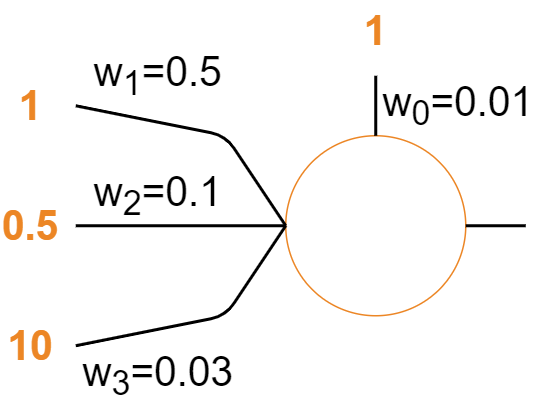
\includegraphics[width=0.6\textwidth]{figures/Tema 3/PropagationExample_1.png}
\end{figure}
\end{frame}

\begin{frame}{Algoritmo de propagación}
La ecuación que define este \alert{proceso} es la siguiente:
\setcounter{equation}{0}
\begin{equation}
    \Large f\left(\sum_{i=0}^{n} W_{i} X_{i}\right)
\end{equation}

\begin{figure}
\centering
    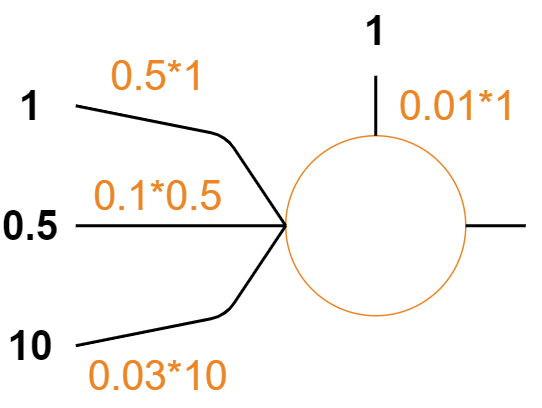
\includegraphics[width=0.6\textwidth]{figures/Tema 3/PropagationExample_2.png}
\end{figure}
\end{frame}

\begin{frame}{Algoritmo de propagación}
La ecuación que define este \alert{proceso} es la siguiente:
\setcounter{equation}{0}
\begin{equation}
    \Large f\left(\sum_{i=0}^{n} W_{i} X_{i}\right)
\end{equation}

\begin{figure}
\centering
    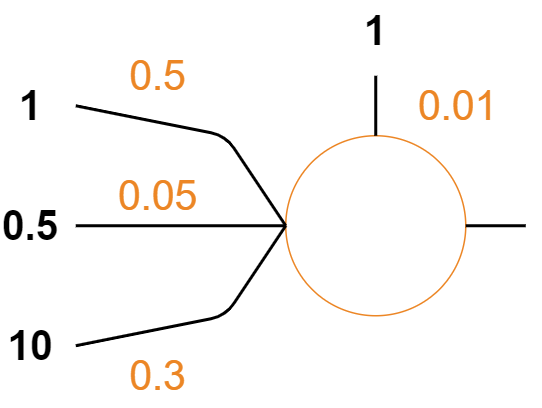
\includegraphics[width=0.6\textwidth]{figures/Tema 3/PropagationExample_3.png}
\end{figure}
\end{frame}

\begin{frame}{Algoritmo de propagación}
La ecuación que define este \alert{proceso} es la siguiente:
\setcounter{equation}{0}
\begin{equation}
    \Large f\left(\sum_{i=0}^{n} W_{i} X_{i}\right)
\end{equation}

\begin{figure}
\centering
    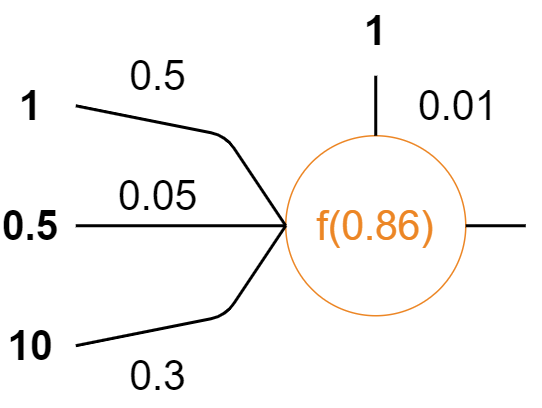
\includegraphics[width=0.6\textwidth]{figures/Tema 3/PropagationExample_4.png}
\end{figure}
\end{frame}

\begin{frame}{Algoritmo de propagación}
La ecuación que define este \alert{proceso} es la siguiente:
\setcounter{equation}{0}
\begin{equation}
    \Large f\left(\sum_{i=0}^{n} W_{i} X_{i}\right)
\end{equation}

\begin{figure}
\centering
    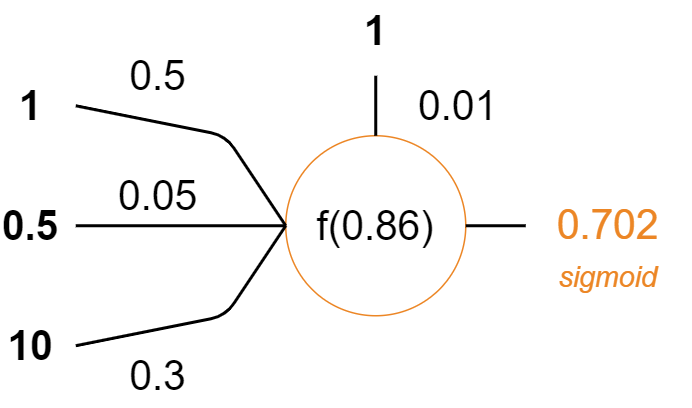
\includegraphics[width=0.8\textwidth]{figures/Tema 3/PropagationExample_5.png}
\end{figure}
\end{frame}

\begin{frame}{Funciones de activación}
Las \alert{funciones de activación} de cada neurona pueden variar, entre las más populares se encuentran:

\begin{figure}
\centering
    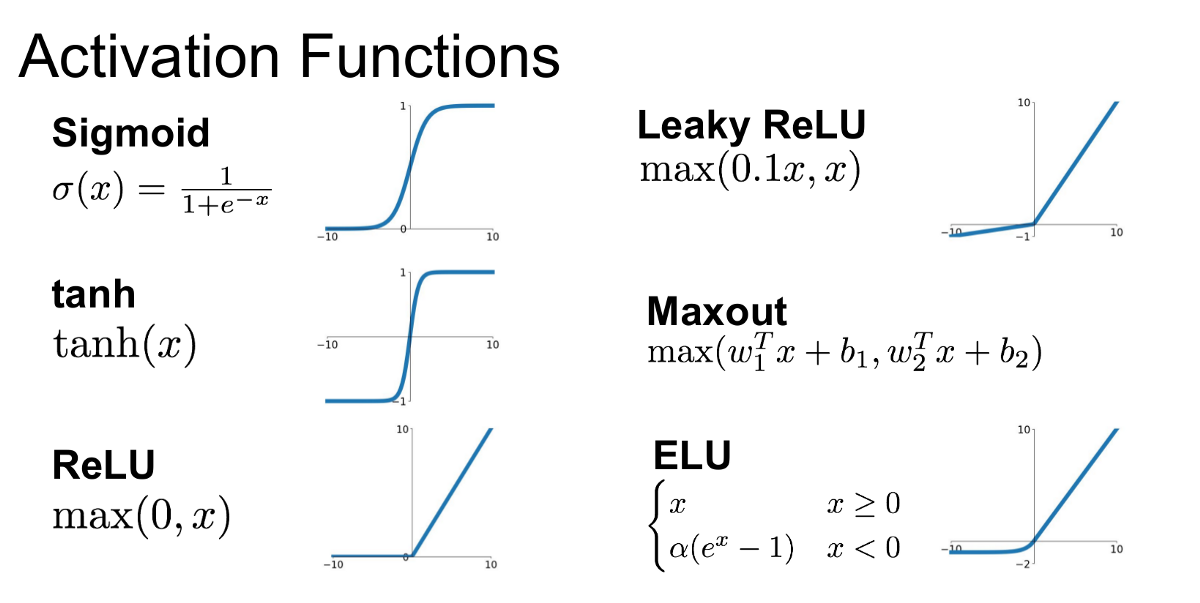
\includegraphics[width=\textwidth]{figures/Tema 3/Activations.png}
    \caption{\cite{Activations}}
\end{figure}
\end{frame}

\begin{frame}{Estructura de capas}
Una red de neuronas \say{estándar} se organiza por \alert{capas}, las cuales se componen por varias \alert{neuronas}.

Cada \alert{capa de neuronas} se conecta con la siguiente y recibe \alert{datos} de la anterior. De esta manera se produce el \alert{flujo de datos} a lo largo de la red.

\begin{figure}
\centering
    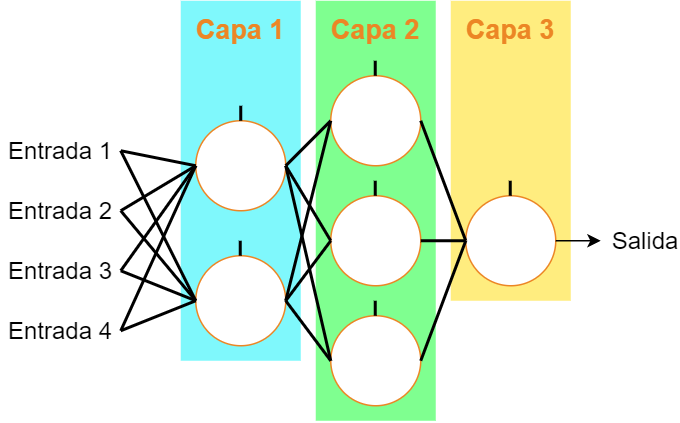
\includegraphics[width=0.8\textwidth]{figures/Tema 3/LayerStructure.png}
\end{figure}
\end{frame}

\begin{frame}{¿Por qué introducir más capas?}
Está matemáticamente \alert{demostrado} que sin función de activación las redes de neuronas sólo son capaces de resolver problemas \alert{linealmente separables}.

Esto es fácilmente demostrable, ya la computación de cada neurona corresponde con la ecuación de \alert{una recta}, y su combinación también.

\begin{figure}
\centering
    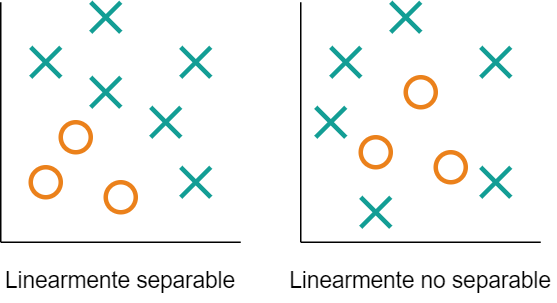
\includegraphics[width=0.5\textwidth]{figures/Tema 1/Separabilidad_Lineal.png}
\end{figure}

Por otra parte, K. Hornik, M. Stinchcombe, y H. White demostraron el 1985 que con \alert{una única capa oculta} las redes neuronales artificiales se convierten en aproximadores universales \cite{hornik1989multilayer}.
\end{frame}


\begin{frame}{Gradient descent y learning rate}
\alert{Descenso de gradiente}: algoritmo de optimización iterativo de primer orden que permite encontrar mínimos \alert{locales} en una función diferenciable. (Wikipedia).

¿Cómo funciona? Derivadas parciales para bajar la pendiente.


\begin{columns}[c]
\centering
\begin{column}{0.33\textwidth}
    \centering
    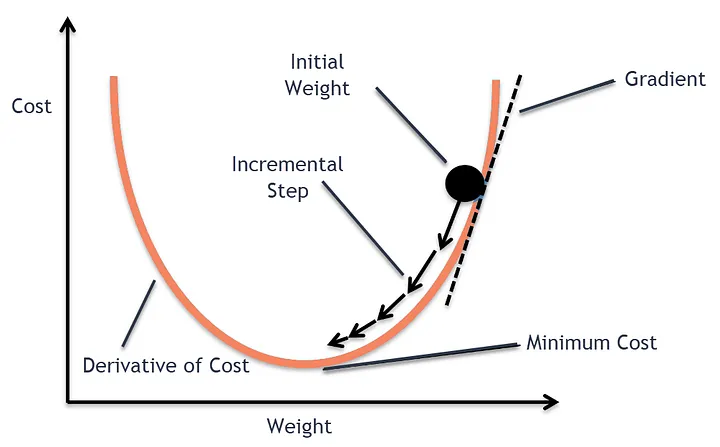
\includegraphics[width=\textwidth]{figures/Introduccion/gradient.png}
\end{column}
\begin{column}{0.33\textwidth}
    \centering
    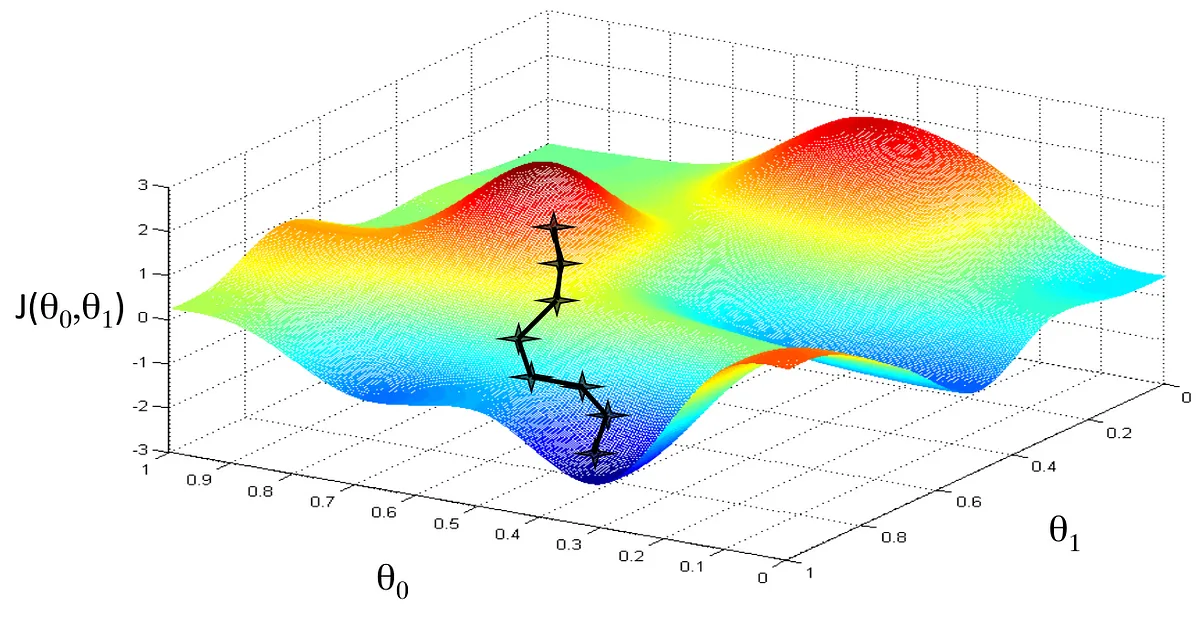
\includegraphics[width=\textwidth]{figures/Introduccion/gradient_3d.png}
    ¡Ojo! pérdida no datos
\end{column}
\begin{column}{0.33\textwidth}
    \centering
    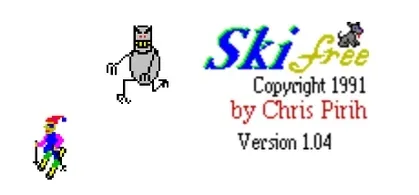
\includegraphics[width=\textwidth]{figures/Introduccion/descenso.png}
\end{column}
\end{columns}


\href{https://www.deeplearning.ai/ai-notes/optimization/index.html\#learning-rate}{Gradient descent un parámetro (batch size y learning rate)}

\href{https://www.deeplearning.ai/ai-notes/optimization/index.html\#adjusting-gradient-descent-hyperparameters}{Gradient descent w y b} y \href{https://www.deeplearning.ai/ai-notes/optimization/index.html\#iterative-update}{Optimizadores}

\centering
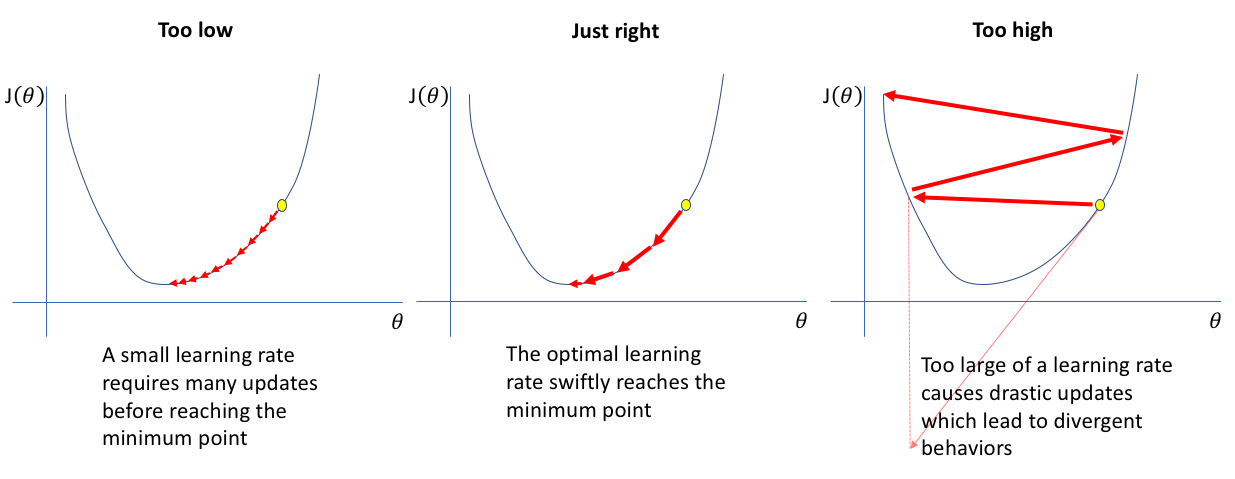
\includegraphics[width=0.7\textwidth]{figures/Introduccion/lr.png}

\end{frame}

\begin{frame}{Algoritmo de retropropagación}
El algoritmo de \alert{retropropagación} o \alert{backpropagation} es el encargado de \alert{adaptar} la red de neuronas a su cometido específico.

Se basa en actualizar los \alert{pesos} de la red dependiendo del \alert{error} que esta haya tenido a la hora de predecir una \alert{salida} en concreto.

Con backpropagation obtendremos los \alert{gradientes (derivadas)} de la función de pérdida
para cada \alert{peso} de cada \alert{capa oculta}.

\begin{equation}
    \bigtriangleup w_i = w_i - \alpha \cdot (Error)
\end{equation}

donde $\alpha$ es el \alert{learning rate}, que define la \alert{magnitud} con la que la red realiza la \alert{actualización} de sus pesos.

\href{https://xnought.github.io/backprop-explainer/}{Backpropagation interactivo}

\end{frame}


\begin{frame}{Funciones de pérdida}
Existen múltiples métodos para calcular la \alert{distancia} de la \alert{predicción $\hat{y}$} con respecto de la \alert{salida deseada $y$}. Es decir, múltiples funciones de pérdida que nos permiten calcular el error.

\begin{equation}
    \textbf{MAE} = \frac{1}{n} \sum{\left | y - \hat{y} \right |}
\end{equation}

\begin{equation}
    \textbf{MSE} = \frac{1}{n}\sum{(y - \hat{y})^2}
\end{equation}

\begin{equation}
    \textbf{Binary Cross-Entropy} = - \left( y \log(\hat{y}) + (1 - y) \log(1 - \hat{y}) \right)
\end{equation} \href{https://www.desmos.com/calculator/hzgt6hyqr3}{Dibujo de la funciónlog.} Condicional if -> $y * ... + (1-y) * ...$

\begin{equation}
    \textbf{Cross-Entropy} = - \sum_{i=1}^{N}{y \cdot  \log \hat{y}}
\end{equation}
\end{frame}

\begin{frame}{Entrenamiento de redes neuronales}
Al realizar un entrenamiento con \alert{modelos de aprendizaje} se realiza una división del \alert{conjunto de datos} con el que se entrena. Este proceso ayuda a comprobar la \alert{fiabilidad} de la red.

\begin{figure}
\centering
    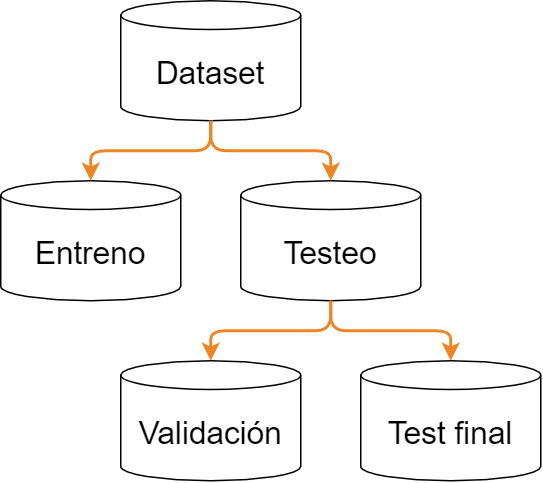
\includegraphics[width=0.6\textwidth]{figures/Tema 3/DatasetDivision.png}
\end{figure}
\end{frame}

\begin{frame}{Bias-variance tradeoff}
Existen dos \alert{métricas} de alto nivel que evalúan el rendimiento de una red neuronal:
\begin{itemize}
    \item \alert{Bias}: Es el error del modelo ante el conjunto de datos de \alert{entrenamiento}.
    \item \alert{Variance}: Es el error del modelo ante el conjunto de datos de \alert{testeo} respecto los de entrenamiento. 
\end{itemize}

\begin{figure}
\centering
    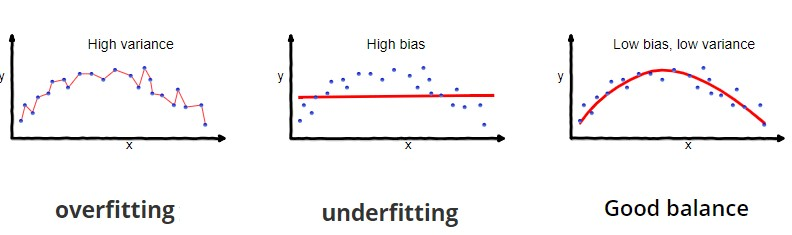
\includegraphics[width=\textwidth]{figures/Tema 3/BiasVariance_1.jpg}
    \caption{\cite{BiasVariance_1}}
\end{figure}
\end{frame}

\begin{frame}{Bias-variance tradeoff}
\begin{figure}
\centering
    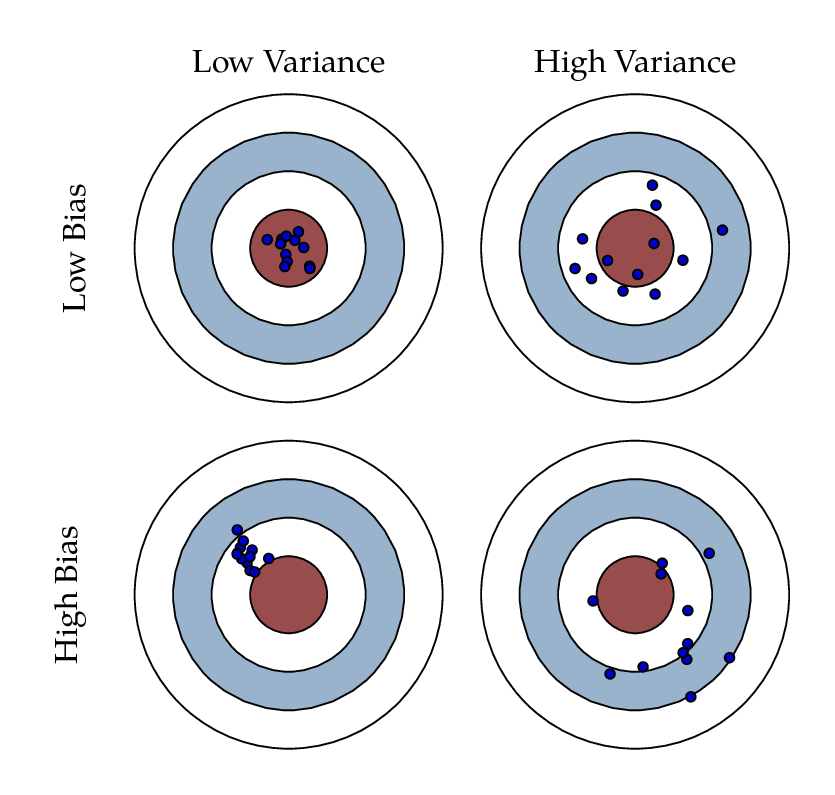
\includegraphics[width=0.7\textwidth]{figures/Tema 3/BiasVariance.png}
    \caption{\cite{BiasVariance}}
\end{figure}
\end{frame}

\begin{frame}{¿Cómo detectar alto bias o variance?}

\begin{columns}[c]
\begin{column}{0.49\textwidth}
\Large \alert{Alto bias}
\end{column}

\begin{column}{0.49\textwidth}
\Large \alert{Alto variance}
\end{column}
\end{columns}

\begin{columns}[c]
\begin{column}{0.49\textwidth}
\begin{itemize}
    \item Underfitting.
    \item Sobre-simplificación del problema.
    \item Valores de pérdida demasiado altos.
    \item Falla al capturar la tendencia de los datos.
\end{itemize} 
\end{column}

\begin{column}{0.49\textwidth}
\begin{itemize}
    \item Overfitting.
    \item Dataset demasiado ruidoso.
    \item Demasiada complejidad.
\end{itemize} 
\end{column}
\end{columns}
\end{frame}

\begin{frame}{Esquema general de entrenamiento de redes neuronales}
\begin{figure}
\centering
    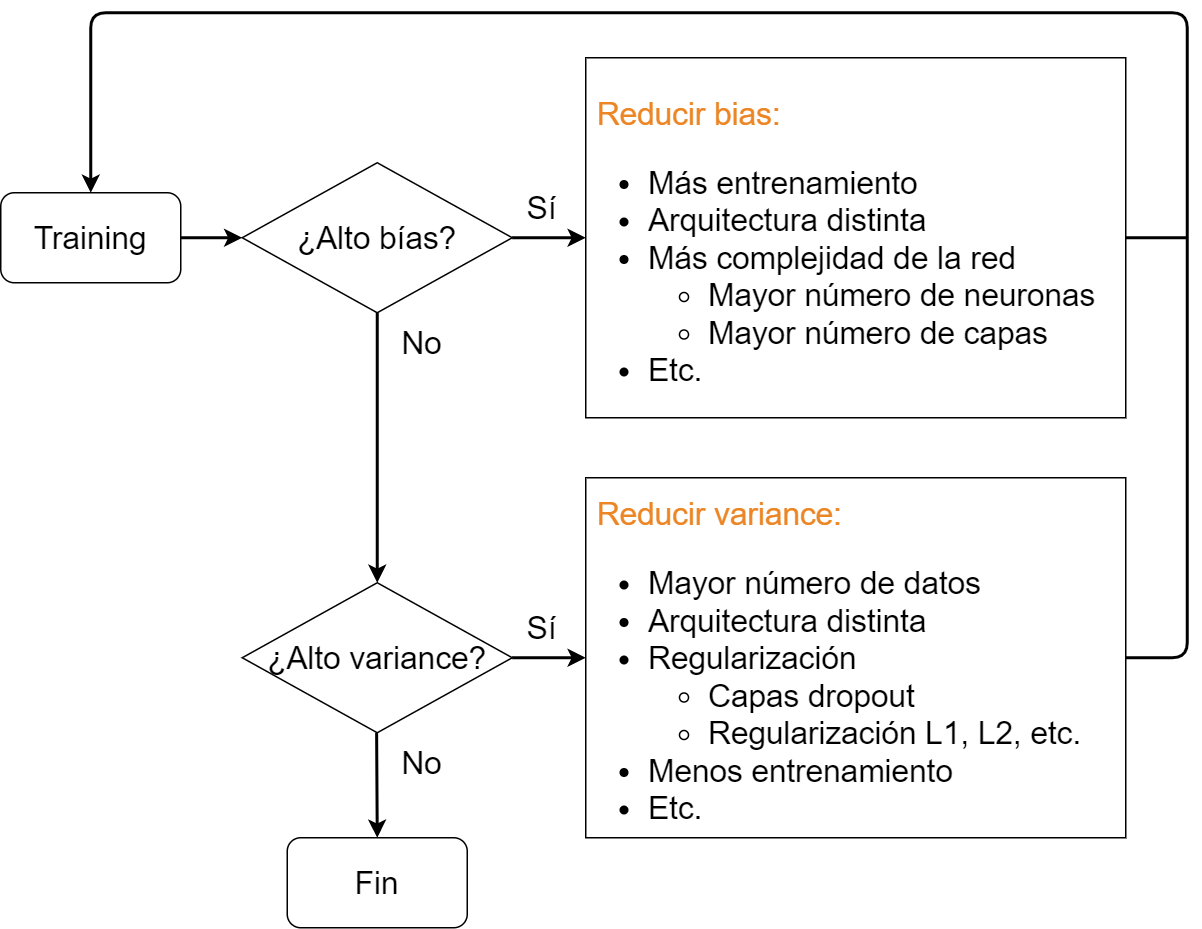
\includegraphics[width=0.9\textwidth]{figures/Tema 3/NNTrainingScheme.png}
\end{figure}
\end{frame}

\begin{frame}{Problemas del gradiente}
Los problemas \alert{derivados del gradiente} son comunes a todas las redes neuronales. Estos están \alert{directamente influenciados} por el número de capas de la red.

Se diferencian dos tipos:
\begin{itemize}
    \item Gradient explosion.
    \item Gradient vanishing.
\end{itemize}

Al realizarse la \alert{retropropagación} los \alert{valores de pérdida} pasan de unas capas a otras. En este algoritmo las derivadas de cada neurona pueden llegar a \alert{descontrolarse}.

\begin{equation}
    W_{x}^{\prime}=W_{x}-\mathrm{\alpha}\left(\frac{\partial \text {Loss}}{\partial W_{x}}\right)
\end{equation}
\end{frame}

\begin{frame}{Problemas del gradiente: Gradient explosion}
\begin{figure}
    \centering
    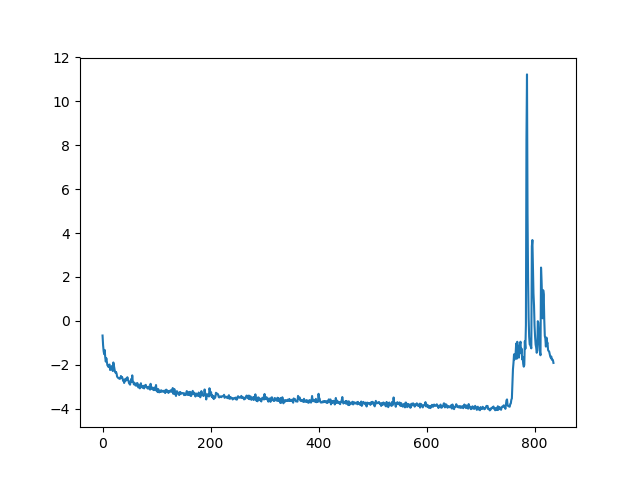
\includegraphics[width=0.6\textwidth]{figures/Tema 3/GradientExplosion.png}
    \caption{\cite{GradienExplosion}}
\end{figure}

El \alert{gradient explosion}, también conocido como \alert{exploding gradients} sucede cuando la actualización de pesos toma valores \alert{muy elevados}.

Se identifica con valores de pérdidas de \alert{NaN o muy exageradas}.
\end{frame}

\begin{frame}{Problemas del gradiente: Gradient Vanishing}
\begin{figure}
    \centering
    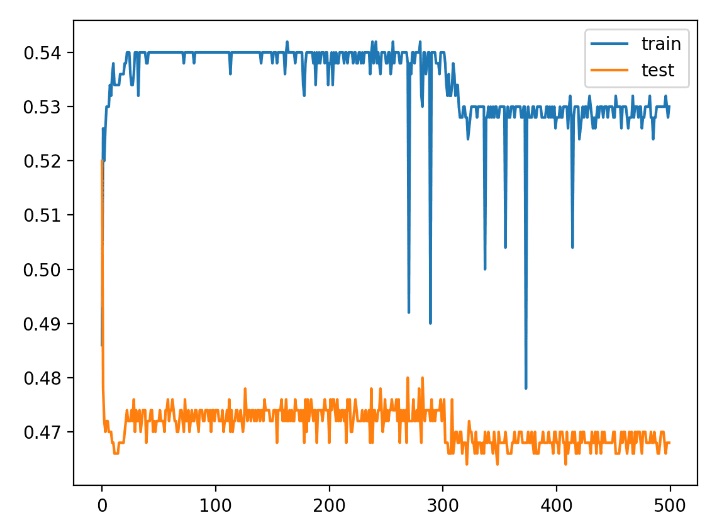
\includegraphics[width=0.6\textwidth]{figures/Tema 3/GradientVanishing.png}
    \caption{\cite{GradienVanishing}}
\end{figure}

Cuando sucede \alert{gradient vanishing}, también llamado \alert{vanishing gradients}, la actualización de pesos se hace \alert{nula} por tener valores \alert{muy pequeños}.

Se identifica cuando la pérdida es \alert{constante en el tiempo}.
\end{frame}

\begin{frame}{Origen de los problemas derivados del gradiente}
La principal \alert{causa} de estos problemas es usar \alert{funciones de activación} cuya derivada \alert{satura a 0}.

\begin{figure}
    \centering
    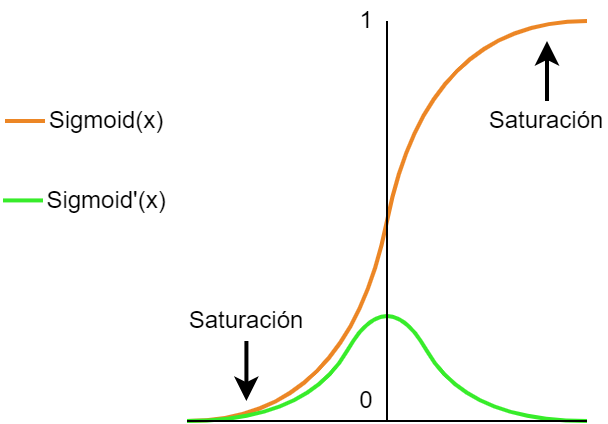
\includegraphics[width=0.6\textwidth]{figures/Tema 3/GradientCause.png}
\end{figure}

Sucede principalmente con las funciones \alert{tanh} y \alert{sigmoid}, por lo tanto se \alert{recomienda} el uso de ReLU para capas ocultas en una red.
\end{frame}

\begin{frame}{Playground}
\begin{figure}
    \centering
    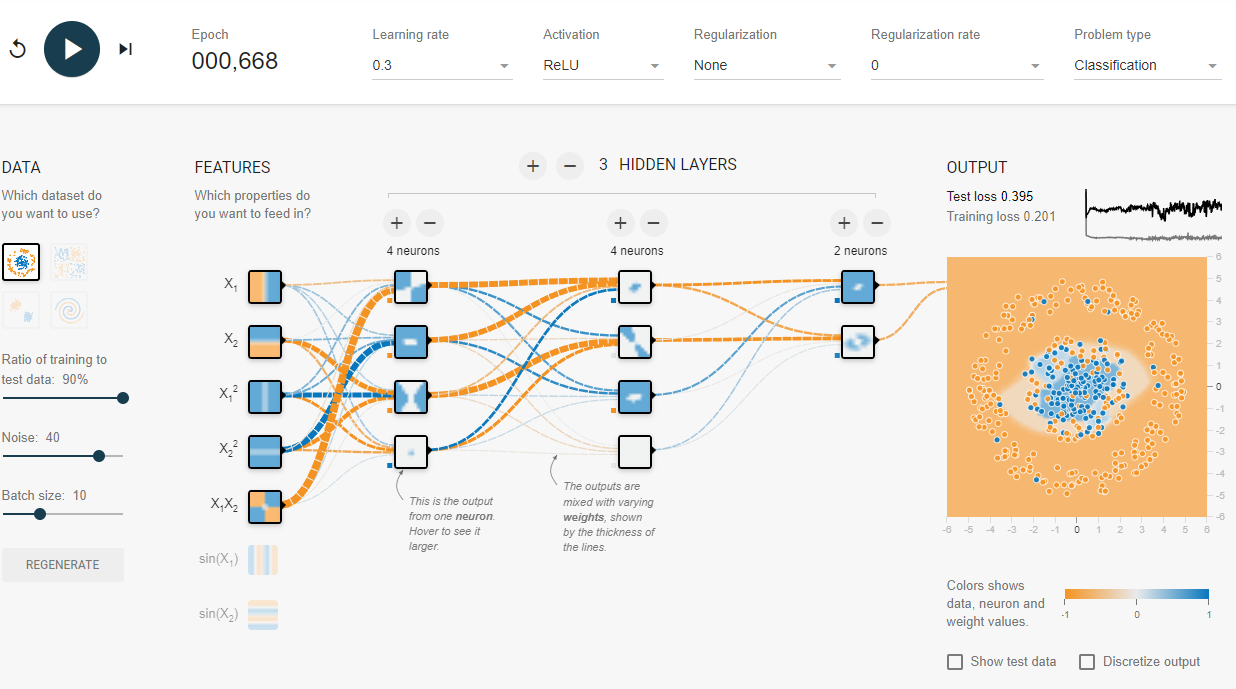
\includegraphics[width=\textwidth]{figures/Tema 3/Playground.png}
    \caption{\href{https://playground.tensorflow.org/}{Tensorflow playground}}
\end{figure}
\end{frame}

\begin{frame}{Notebook de ejemplo, perceptrón clasificador}
El siguiente notebook contiene un ejemplo de clasificador usando un perceptrón multicapa como red neuronal.

\begin{figure}
    \centering
    
\includegraphics[width=0.4\textwidth]{figures/GoogleColab.png}
\end{figure}
\begin{itemize}
    \centering
    \item {\Large \href{https://colab.research.google.com/drive/1qzLr3sWe4Nk7LW9Jycb9vq-Offsg1yHL?usp=sharing}{1.1\_1-PerceptronClasificador.ipynb}}
\end{itemize}
\end{frame}

\section{Perceptrón multicapa para procesar imágenes}

\begin{frame}{¿Cómo procesar imágenes?}
La idea más \alert{básica} para procesar imágenes con redes neuronales es  transformar la \alert{matriz numérica} de datos a un \alert{vector unidimensional}.

\begin{figure}
    \centering
    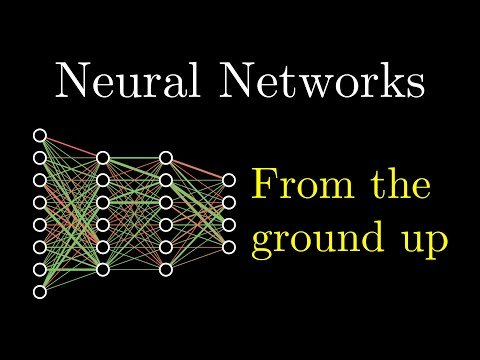
\includegraphics[width=0.7\textwidth]{figures/Tema 3/NNVideo.jpg}
    \caption{\href{https://www.youtube.com/watch?v=aircAruvnKk&t=218s}{Vídeo youtube}}
\end{figure}
\end{frame}

\begin{frame}{Capa de reshape}
La capa de \alert{keras} llamada \say{\alert{reshape}} se encarga de realizar esa transformación de \alert{matriz} a \alert{vector}.

Sin embargo el principal \alert{inconveniente} al tratar las imágenes de esta manera es la \alert{pérdida total} de información espacial de la imagen.
\end{frame}


\begin{frame}{Notebook de ejemplo, perceptrón clasificador de imágenes}
El siguiente notebook contiene un ejemplo de clasificador de imágenes usando un perceptrón multicapa como red neuronal.

\begin{figure}
    \centering
    
\includegraphics[width=0.4\textwidth]{figures/GoogleColab.png}
\end{figure}
\begin{itemize}
    \centering
    \item {\Large \href{https://colab.research.google.com/drive/1h2cas9zCyUsutVJrJwR43zJMzOurunoV?usp=sharing}{1.1\_2-PerceptronImagenes.ipynb}}
\end{itemize}
\end{frame}
\addcontentsline{toc}{section}{Referencias}

\begin{frame}[allowframebreaks]{Referencias}
    \bibliographystyle{unsrt}
    \bibliography{references.bib}
\end{frame}

\end{document}